In this section, we discuss the performance and scalability of a
gravitational $N$-body simulation code implemented using FDPS. The
code is essentially the same as the sample code described in
section~\ref{sec:samplecode}, except for the following two differences
in the user code for the calculation of the interaction. First, here,
we used the expansion up to quadrupole moment, instead of
monopole-only one used in the sample code, to improve the
accuracy. Second, we used highly-optimized kernel developed using SIMD
builtin functions, instead of the simple one in the sample code.

We apply this code for the simulation of the Milky Way-like galaxy,
which consists of a bulge, disk, and dark matter halo.  For the review
of dynamics within galaxies, see
\cite{2014PASA...31...35D}. For examples of recent large-scale
simulations, see \cite{2011ApJ...730..109F, Bedorf:2014:PGT:2683593.2683600}.

The initial condition is the Milky Way model, the same as that
in \cite{Bedorf:2014:PGT:2683593.2683600}, consisting of a bulge,
disk, and dark matter halo.  The mass of the bulge is $4.6 \times 10^9
M_\odot$ (solar mass), and it has a spherically-symmetric density
profile of a Hernquist density profile \cite{1990ApJ...356..359H} with
the half-mass radius of $0.5$~kpc. The disk is an axisymmetric
exponential disk with the scale radius of $3$~kpc, scale height of
$200$~pc and mass $5.0 \times 10^{10}M_\odot$. The dark halo has an
Navarro-Frenk-White (NFW) density profile \cite{1996ApJ...462..563N}
with the half-mass radius of $40$~kpc and mass of $6.0 \times 10^{11}
M_\odot$. In order to realize the Milky Way model, we actually use
GalacticICS \cite{2005ApJ...631..838W}.
We also show the result for the Plummer
model \cite{1911MNRAS..71..460P}. 

\begin{figure}
  \begin{center}
    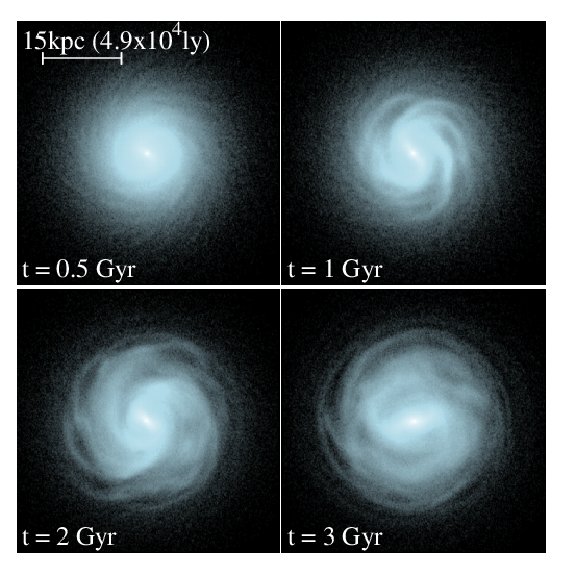
\includegraphics[width=8cm]{fig/disk.eps}
  \end{center}
  \caption{Face-on surface density maps of the bulge and disk. The
  total number of particles is $0.97$ billions. }
  \label{fig:evolutiondisk}
\end{figure}

We adopt $\theta=0.4$ for the opening angle for the tree algorithm. In
this paper, we present the weak-scaling performance of the code with
FDPS. Therefore we fixed the number of particles per node to $2.1$
million and measured the performance for number of nodes in the range
of 128 to 16384.  For the Plummer model, performance measurement for up
to $76544$ has been finished at the time of writing. The obtained
performance numbers are quite similar for these two models.

Figure~\ref{fig:evolutiondisk} illustrates the time evolution of the
bulge and disk in the run with $512$ nodes. The disk is initially
axisymmetric.  We can see that spiral structure develops (0.5 and 1
Gyrs) and central bar structure follows the spiral (1Gyrs and
later). As the bar grows, the two-arm structure becomes more visible
(3Gyrs).

Figure~\ref{fig:benchdisk} shows the measured performance. We can see
the measured efficiency and scalability are both very good. Efficiency
is very close to 50\%, for both models and for the entire range of
nodes. Wallclock time shows slight  increase for larger number of nodes,
but this is due to the increase of the calculation cost and not due to
the degradation of the efficiency. 

B\'edorf \textit{et al.}\cite{Bedorf:2014:PGT:2683593.2683600}
reported the wallclock time of 4 seconds for their 27-billion particle
simulation on the Titan system with 2048 NVIDIA Tesla K20X, with the
theoretical peak performance of 8PF (single precision, since single
precision us used for interaction calculation). This corresponds to
0.8 billion particles per second per petaflops. Our code on K computer
requires 15 seconds on 16384 nodes (2PF theoretical peak), resulting in
1 billion particles per second per petaflops. Therefore, we can
conclude that our FDPS code achieved the performance slightly better
than one of the best codes specialized to gravitational $N$-body
problem.

\begin{figure}
  \begin{center}
    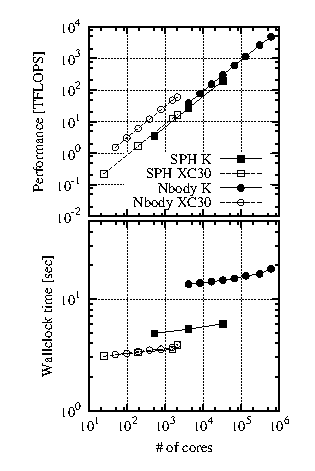
\includegraphics[width=8cm]{fig/bench.eps}
  \end{center}
  \caption{Performance measured in the speed of the floating-point
    operation (top) and wallclock time per one timestep (bottom)
    plotted as functions of the number of nodes. In the bottom panel,
    time spent for interaction calculation (IC), and domain
    decomposition plus exchange particles (DD+EP) are also shown.  In
    both panels, circles and crosses indicate the Milky Way (MW)
    and Plummer (PL) models.
    }
  \label{fig:benchdisk}
\end{figure}

% LocalWords:  FDPS superparticle monopole quadrupole SIMD builtin Hernquist IC
% LocalWords:  Frenk NFW EP scalability TPP PFLOPS NVIDIA kpc axisymmetric pc
% LocalWords:  GalacticICS Gyrs timestep edorf et al petaflops Wallclock
% LocalWords:  wallclock
